% Asset ID: A21BinomialExpansionTikZ-002
% Unit: A21
% Topic code: A21-SS
% Topic ID: A21BinomialExpansion
% Purpose: Coefficient pattern for rational binomial expansion
\documentclass[tikz,border=10pt]{standalone}
\usepackage{amsmath}
\usetikzlibrary{arrows.meta,positioning}
\begin{document}
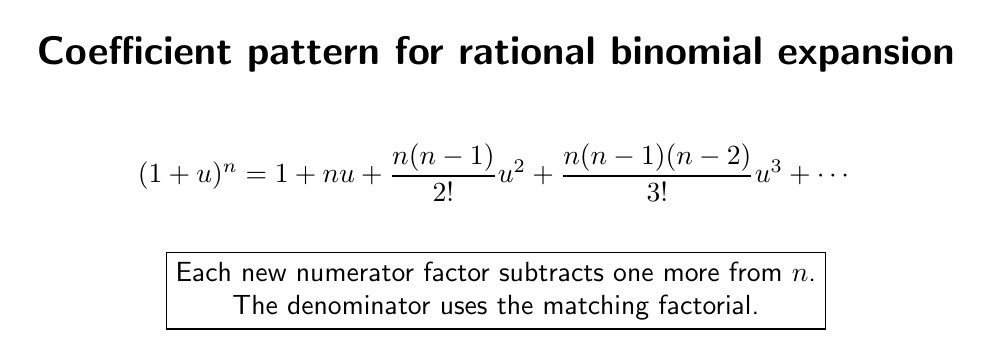
\begin{tikzpicture}[every node/.style={font=\sffamily}]
\node[font=\sffamily\bfseries\Large] at (0,3) {Coefficient pattern for rational binomial expansion};
\node[align=center] at (0,1.5) {$ (1+u)^n=1+nu+\dfrac{n(n-1)}{2!}u^2+\dfrac{n(n-1)(n-2)}{3!}u^3+\cdots $};\node[draw,align=center] at (0,0) {Each new numerator factor subtracts one more from $n$.\\The denominator uses the matching factorial.};
\end{tikzpicture}
\end{document}
